\documentclass[aps,pra, twocolumn]{revtex4-1}

\usepackage{graphicx,epstopdf}
\usepackage{amsmath}
\usepackage{mathtools}
\usepackage{mathrsfs}


\begin{document}


\title{On the dynamics of gravitational stability in protoplanetary disks}

\author{Evan Anders}
\affiliation{Department of Physics, Whitworth University, 300 W. Hawthorne Rd., Spokane, WA 99251}


\date{\today}

\begin{abstract}
Protoplanetary disks are observed astrophysical objects which surround young stars and are generally modeled as geometrically thin cylinders.  Here we create a framework for describing the dynamics of these disks, starting from base principles and utilizing conservation laws.  After creating this framework, we examine gravitational and centripetal forces as well as random motions of disk constituents to characterize gravitational stability in these disks.  A brief discussion of the outcomes of instability focusing on  fragmentation and planet formation follows.
\end{abstract}



\maketitle


\section{\label{section1} Introduction}

Protoplanetary disks are disks of gas and dust which surround young stars, display early conditions of planet formation, and typically display lifetimes on the order of $10^6$ years.  Their masses are far lower than the mass of their star and their composition and behavior is distinctly different from that of debris disks surrounding older stars.  Consequently, it is exceptionally rare to observe the evolution of these disks.  Rather, statistical studies of populations and computational simulations provide insight on their behavior and development, with angular momentum conservation proving to be at the heart of their slow evolution.   \cite{armitage2011}

A large body of the work that has been published on such disks pertains to basic topics of classical mechanics.  Gravitation and gravitational instability, as well as non-inertial reference frame dynamics, have offered insight on disk evolution and have helped informed a large portion of the literature throughout the past decades.  In certain regimes, it is possible to model the disk using such base principles and show that planetary formation can occur.  This focus of this paper is on developing a schema with which to describe protoplanetary disks and evaluate their stability based on simple classical interactions.  In section \ref{section 2}, we will develop a thorough system for describing the movement and temperature of disk constituents.  In section \ref{section 3}, the effects of gravity and the centripetal force, alongside random particle motions, will be considered to understand what causes gravitational instability; a brief discussion of the results of such instability follows.  While there are a number of other, more complex phenomenon involved in disk evolution, such as magnetorotational instability and convection, they are outside of the scope of this paper.



\section{\label{section 2} A schema for the description of disk evolution}
\begin{figure} [b!]
	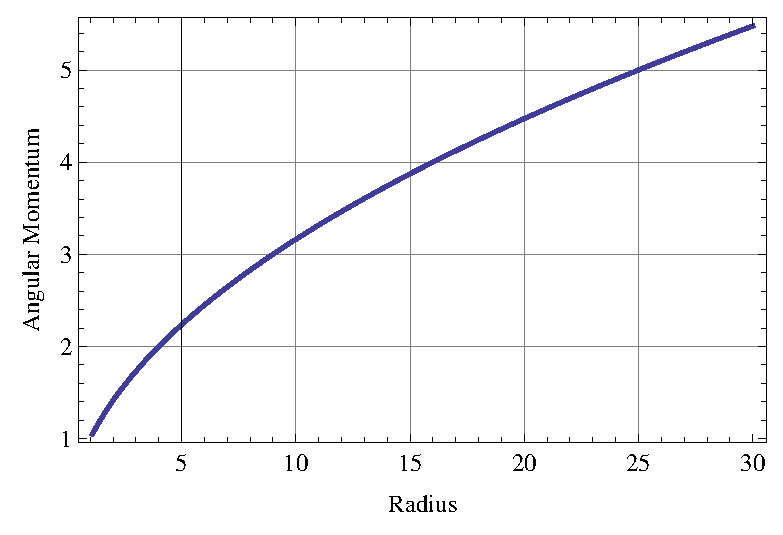
\includegraphics[width=3in]{angularMomentum.eps}
	\caption{This figure qualitatively describes particle angular momentum in protoplanetary disks with respect to increasing radius by using nonspecific values of variables and constants, i.e. $m_p = G = M_* = 1$.  As described in Eq. (\ref{angMomEq}), $\ell \propto \sqrt{r}$. \label{angMom}}
\end{figure}


Protoplanetary disks are modeled as thin cylinders in cylindrical polar coordinates $(r, \phi, h)$.  The thin nature of the disks leads naturally to the assumption that $h_{\text{max}} \ll r_{\text{max}}$.  This assumption, alongside the fluid nature of the disk, whose constituents are gas and dust particles, requires that the mass of the disk be significantly lower than that of the star, or $M_{\text{disk}} \ll M_{*}$.  

In accordance with these assumptions, we model each gas or dust particle at some arbitrary radius $r$ as having some small amount of mass, $m_p$.  Such small particles experience the gravitational pull of their star, which can be modeled  as a point mass at the center of the disk \cite{armitage2011}.  For such particles, we obtain the radial equation of motion \cite{taylor2005},
\begin{equation}
m_p \vec{a}_r = m_p ( \ddot{r} - r\dot{\phi}^2 )\hat{r} = - \frac{G M_* m_p}{r^2}\hat{r} . \label{rMotion}
\end{equation}
Assuming that the disk is not rapidly collapsing inwards or expanding outward, we can model it as a thin accretion disk.  Solving Eq. (\ref{rMotion}) for the Keplerian angular velocity under the assumption that $\ddot{r} = 0$, we find \cite{armitage2011}
\begin{equation}
 \Omega_K = \dot{\phi} = \sqrt{\frac{G M_*}{r^3}}.
\end{equation}
Consequently, the angular momenta of the disk particles can be simply expressed using base principles, where \cite{taylor2005},
\begin{equation}
\ell = \left| \vec{r} \times \vec{p} \right| = m_p r^2 \Omega_K = m_p \sqrt{G M_* r}, \label{angMomEq}
\end{equation}
which clearly describes an increase in particle angular velocity proportional to $\sqrt{r}$, as shown in Fig. \ref{angMom}.  

Maintaining the assumption that protoplanetary disks are accretion disks, it is necessary to account for the angular momentum which is lost among the disk constituents.  There are two possible mechanisms for this loss of angular momentum: (i) the momentum is redistributed within the disk or (ii) the momentum is lost to an external sink \cite{armitage2011}.  This paper is concerned with the former, with respect to how the gravity of the star and neighboring particles affect the motion of disk constituents.



\subsection{\label{section2.1} A model of evolution in accretion disks }
Among thin disks as described in the previous section, the vertical structure of the disk is insignificant.  Integrating over this thickness yields a surface mass density, $\mu(r, t)$, which is independent of height  \cite{armitage2011}.  Assuming that our disk is an accretion disk, it is essential for there to be some radial `drift' velocity, $u_r$, in addition to the primary azimuthal velocity,
\begin{equation}
u_\phi = r\Omega_K. \nonumber
\end{equation}
The drift velocity, $u_r$ is negative close to the star, depends upon both $r$ and $t$, and is characterized by the surface density $\mu$.

In order to understand the evolution behavior of the disk, we must examine an infinitesimally thin ring between some radii, $R$ and $R + dr$.  This ring has a total mass of $M_\text{ring} = \pi \left(2 R dr + dr^2 \right)\mu \approx (2 \pi R \mu) dr$ and, therefore, a total angular momentum of $\ell_\text{ring} = (2\pi R^3 \mu \Omega_K)dr$ \cite{king2002}.


\subsubsection{\label{section 2.1.1} Conservation of mass}
According to the principle of conservation of mass, it is necessary for any change in the mass of our thin ring to be a direct result of mass flowing into or out of the neighboring sections of the disk.  Thus we can solve for the change of mass of the ring,
\begin{equation}
\begin{split}
\frac{\partial}{\partial t}\left(  M_\text{ring}\right)= M_{\text{in}}(R) + M_{\text{in}}&(R + dR)  \\
= 2\pi [ R u_r(R, t) \mu&(R, t) -   \\
(R + dR)& u_r(R+dR, t) \mu(R+dR, t)] \\
 \approx -2\pi dR \,\frac{\partial}{\partial r}\,(\,R&\mu u_r\,).
\nonumber
\end{split}
\end{equation}
This provides the mass conservation equation of the disk in the limit $dr \rightarrow 0$, where
\begin{equation}
\frac{\partial}{\partial t}\left(  2\pi R  \mu dr \right) + 2\pi dr \frac{\partial}{\partial r}(R \mu u_r) = 0. \nonumber
\end{equation}
Generalizing from the specific case at $R$ to any arbitrary $r$, the equation of conservation of mass within a protoplanetary accretion disk is \cite{king2002},
\begin{equation}
r \frac{\partial \mu}{\partial t} + \frac{\partial}{\partial r}(r \mu u_r) = 0. \label{consMass}
\end{equation}


\subsubsection{\label{section 2.1.2} Conservation of angular momentum}
It is natural to approach conservation of angular momentum in manner similar to that which was used in determining the governing equation for the disk's conservation of mass. In addition to accounting for the flow of mass in an out of our thin ring, we must also account for a term which relates to the change caused by viscous torques, $\Gamma(r, t)$, and we find that
\begin{equation}
\frac{\partial}{\partial t}\left( \ell_{\text{ring}} \right) \approx  -2\pi dr \frac{\partial}{\partial r}(R^3 \mu u_r \Omega_K) + \frac{\partial \Gamma}{\partial r}dr.
\nonumber
\end{equation}
By isolating common terms, generalizing $R$ to $r$, and taking the limit as $dr \rightarrow 0$, we find the disk's governing equation for conservation of angular momentum \cite{king2002},
\begin{equation}
r \frac{\partial}{\partial t} (\mu r^2 \Omega_K) + \frac{\partial}{\partial r} (r^3 \mu u_r  )\Omega_K' = \frac{1}{2\pi} \frac{\partial \Gamma}{\partial r}, \label{consAng}
\end{equation}
where
\begin{equation}
\Omega_K' = \frac{\partial \Omega_K}{\partial r}. \nonumber
\end{equation}


\subsubsection{\label{section 2.1.3} Governing equation for surface density time evolution}
Using Eq. (\ref{consMass}) and assuming that $\Omega_K' = 0$, Eq. (\ref{consAng}) becomes
\begin{equation}
R\mu u_r \frac{\partial}{\partial r} (R^2 \Omega_D) = \frac{1}{2\pi} \frac{\partial \Gamma}{\partial r}.
\end{equation}
Combining this result once again with Eq. (\ref{consMass}), it is possible to eliminate $u_r$, finding
\begin{equation}
R \frac{\partial \mu}{\partial t} = -\frac{\partial}{\partial r}(R \mu u_r) = - \frac{\partial}{\partial r}\left[ \frac{1}{2\pi \frac{\partial}{\partial r}(R^2)\Omega_K'}\frac{\partial \Gamma}{\partial r} \right]. \label{EqMotion1}
\end{equation}

In the case of an accretion disk with randomly moving particles, the flow of mass into and out of a region will create a change in angular momentum via a viscous torque.  Throughout the disk, we find that the torque per unit arc length follows the form \cite{king2002}
\begin{equation}
\gamma(r, t) = \nu \mu r^2 \Omega_K'. \nonumber
\end{equation}
The total torque acting on any infinitely thin ring of radius $r$ naturally takes on the form
\begin{equation}
\Gamma(r, t) = 2 \pi r \gamma(r, t) = 2 \pi \nu \mu r^3 \Omega_K, \label{torque}
\end{equation}
with which Eq. (\ref{EqMotion1}) can be solved.  The equation of motion for masses within the disk takes on the form
\begin{equation}
\frac{\partial \mu}{\partial t} = \frac{3}{r} \frac{\partial}{\partial r} \left| r^{1/2}\frac{\partial}{\partial r}\left( \nu \mu r^{1/2} \right) \right|
\end{equation}
so long as torques external to the disk system and mass losses are neglected\cite{king2002, armitage2011}.  This follows directly from conservation of mass and angular momentum for a viscous fluid with kinematic viscosity $\nu$.


\subsection{\label{section 2.2} Characteristics of steady-state thin disks}
For a disk system in which external conditions change at timescales much longer than the radial structure of the disk itself changes, we can set time derivatives from our previous conservation equations, Eqs. (\ref{consMass}) \& (\ref{consAng}), equal to zero.  In such a steady state, Eq. (\ref{consMass}) yields
\begin{equation}
R\mu u_r = \text{constant}, \nonumber
\end{equation}
from which it is easy to see that the total change of mass of the disk--the accretion rate of the disk--takes on the form
\begin{equation}
\dot{M} = -2\pi R \mu u_r, \label{modifiedMass1}
\end{equation}
where the negative sign arises as a result of the fact that $u_r$ is in the inward radial direction.  In steady state, Eq. (\ref{consAng}) yields
\begin{equation}
R^3 \mu u_r \Omega_K = \frac{\Gamma}{2\pi} + \frac{C}{2\pi} \nonumber
\end{equation}
for some constant $C$.  Plugging in Eq. (\ref{torque}) and rearranging, it is clear that \cite{king2002}
\begin{equation}
- \nu \mu \Omega_K' = -\mu u_r \Omega_K  + \frac{C}{2\pi R^3 }. \label{modifiedAng1}
\end{equation}


\subsubsection{\label{section 2.2.1} Relating mass flow, viscosity, and mass density}
\begin{figure} [b!]
	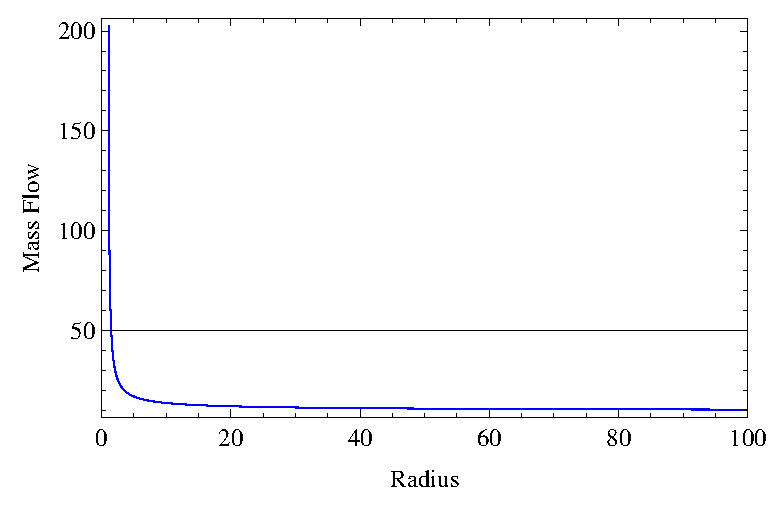
\includegraphics[width=3in]{massFlow.eps}
	\caption{This figure qualitatively describes the relationship between mass flow rate and radius.  This plot was created using Eq. (\ref{massFlow}) with nonspecific values of other variables ($\nu = \mu = R_* = 1$).  Clearly, mass flow is very large near the star.  At further radii, this flow quickly drops off to a very low, roughly asymptotic value. \label{massFlowFig}}
\end{figure}
\begin{figure} [b!]
	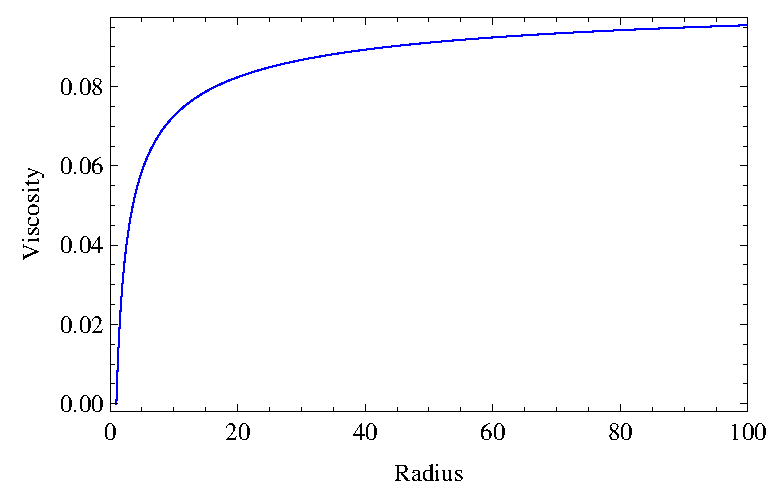
\includegraphics[width=3in]{viscosity.eps}
	\caption{This figure qualitatively describes the relationship between viscosity and radius.  This plot was created using Eq. (\ref{massFlow}) with nonspecific values of other variables ($\dot{M} = \mu = R_* = 1$).  At radii near the star, the viscosity increases rapidly.  At further radii, it flattens out and approaches an asymptotic value. \label{viscosityFig}}
\end{figure}
\begin{figure} [t!]
	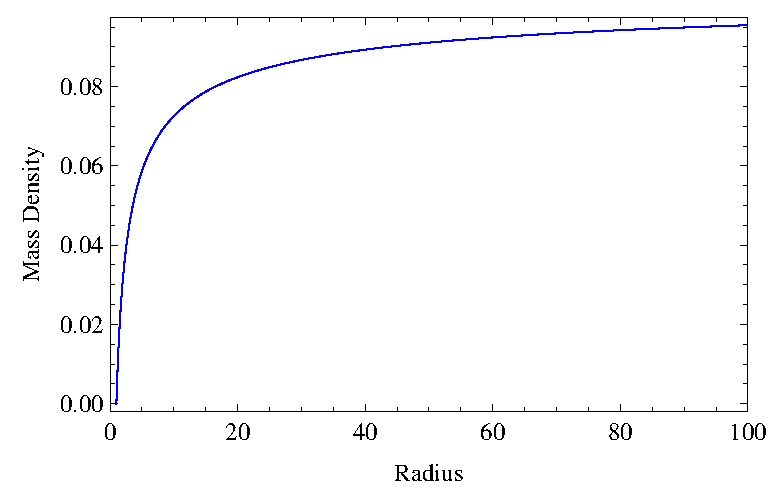
\includegraphics[width=3in]{massDensity.eps}
	\caption{This figure qualitatively describes the relationship between mass density and radius, and was created using Eq. (\ref{massFlow}) with nonspecific values of other variables ($\dot{M} = \nu = R_* = 1$).  Clearly, as evidenced by the parallelism of $\nu$ and $\mu$ in Eq. (\ref{massFlow}), this follows the same relationship described in Fig. \ref{viscosityFig}.  \label{massDensityFig}}
\end{figure}
Typical stars rotate less rapidly than the Keplerian velocity of the disk.  Thus,
\begin{equation}
\Omega_* < \Omega_K\bigg|_{R_*}. \nonumber
\end{equation}
Now imagine that the particles of the protoplanetary disk extends radially inward so as to be continuous up to the surface of the star.  The difference in angular velocity between the disk constituents and the star requires that angular momentum be lost as the radial drift velocity pulls particles into the star.  This requires a boundary layer of thickness $b$ in which the disk's material falls from the angular velocity of $\Omega_K$ to $\Omega_*$.  

Typically, $b \ll R_*$ and, therefore, $\Omega$ is extremely close to its typical Keplerian value where $\Omega' = 0$.  At this point,
\begin{equation}
\Omega(R_* + b) = \left(\frac{GM_*}{{R_*}^3} \right)^{1/2} \left[1 + X(b/R_*) \right], \label{nearStarOmega}
\end{equation}
where $X[b/R_*]$ is some small fraction.  In this regime, we must evaluate Eq. (\ref{modifiedAng1}), which takes on the form
\begin{equation}
C = 2\pi R_*^3 \mu u_r \Omega(R_* + b) \nonumber
\end{equation}
around the point $R_* + b$.  Combining this result with Eq. (\ref{nearStarOmega}), the constant, $C$,  is determined to be
\begin{equation}
C = - \dot{M}(G M R_*)^{1/2}. \nonumber
\end{equation}
Using the constant determined by our boundary conditions along with Eq. (\ref{modifiedAng1}), we find that
\begin{equation}
\nu \mu = \frac{\dot{M}}{3\pi}\left[ 1 - \sqrt{\frac{R_*}{r}} \right], \label{massFlow}
\end{equation}
which provides a governing equation for the relation between mass flow, viscosity, and surface density in a steady state disk.  The manner in which these variables vary with respect to radius is qualitatively shown in Figs. \ref{massFlowFig}, \ref{viscosityFig}, \& \ref{massDensityFig}.

\subsubsection{\label{section 2.2.2} Disk effective temperature}
Returning momentarily to an arbitrary ring of thickness $dr$, it is necessary to acknowledge that there are competing torques on the inner and outer edge of the ring, following the form
\begin{equation}
\Gamma(r + dr) - \Gamma(r) = \frac{\partial \Gamma}{\partial r}dr \nonumber.
\end{equation}
As this torque aligns with angular momentum, it is possible to utilize the product rule of derivatives to find the rate at which this torque works on our disk,
\begin{equation}
\Omega\Gamma(r + dr) - \Gamma(r) = \left[ \frac{\partial}{\partial r}(\Gamma\Omega) - \Gamma\Omega' \right]dr. \nonumber
\end{equation}
The first of the right-hand terms corresponds to the 'convection' of rotational energy throughout the disk, whereas the $-\Gamma\Omega' dr$ term corresponds to the rate at which mechanical energy is lost.  Due to the geometry of the disk, this energy must be radiated from the top and bottom surfaces, each of which has a surface area of approximately $(2\pi r)dr$. Dividing the dissipated energy by the total surface area from which it radiates, we find an expression for the disk's total viscous dissipation \cite{king2002},
\begin{equation}
D(r) = \frac{\Gamma \Omega'}{4\pi r}= \frac{1}{2}\nu \mu (r\Omega')^2.
\end{equation}
Substituting this finding into Eq. (\ref{massFlow}) yields
\begin{equation}
D(r) =\frac{1}{2}\frac{\dot{M}}{3\pi}\left[ 1 - \sqrt{\frac{R_*}{r}} \right] (r\Omega')^2. \nonumber
\end{equation}
Setting $\Omega = \Omega_K$ and using
\begin{equation}
r\frac{\partial\Omega_K}{\partial r} = -\frac{3}{2}\sqrt{\frac{G M_*}{r^3}}, \nonumber
\end{equation}
it is determined that
\begin{equation}
D(r) = \frac{3GM_*\dot{M}}{8\pi r^3}\left[ 1 - \sqrt{\frac{R_*}{r}} \right].
\end{equation}

At this point it is necessary to acknowledge another assumption regarding the nature of protoplanetary disks: that is, they are optically thick in the $z$-direction.  Accordingly, the disk radiates like a blackbody according to the Stefan-Boltzmann law, which states that energy flux is proportional to the fourth power of absolute temperature,
\begin{equation}
E_{\text{flux}} = \sigma T^4,
\end{equation}
where $\sigma$ is the Stefan-Boltzmann constant.  For a protoplanetary disk, $E_\text{flux} = D(r)$, and the temperature of the disk can be expressed according to \cite{armitage2011, king2002}
\begin{equation}
T(r) = \left( \frac{3GM_*\dot{M}}{8\pi r^3 \sigma}\left[ 1 - \left( \frac{R_*}{r}\right)^{1/2}\right] \right)^{1/4}. \label{tempEq}
\end{equation}
A qualitative description of the variance of temperature with respect to radius can be found in Fig. \ref{tempFig}.


\subsection{\label{section2.3} Disk viscosity models}
\begin{figure} [b!]
	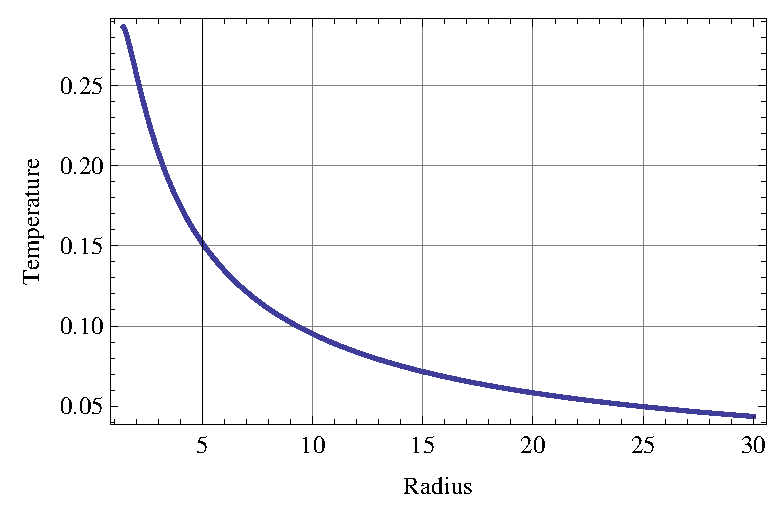
\includegraphics[width=3in]{temperature.eps}
	\caption{This figure qualitatively describes the temperature of a disk with respect to radius, as described by Eq. (\ref{tempEq}), using non-specific values of $M_* = \dot{M} = \sigma = R_* = 1$.  As would be expected, the temperature of the disk is high near the star, and falls off rapidly to a low asymptotic value as the radius increases. \label{tempFig}}
\end{figure}
While the assumptions of local disk turbulence and a lack of external torques acting on the disk have proven useful in yielding the temperature profile of the disk, in order to further predict disk behavior it is necessary to specify the disk's viscosity, $\nu$.  The classical approach at such a point is to assume that
\begin{equation}
\nu = \alpha \frac{c_s^2}{\Omega_K} = \alpha c_s h , \label{nuRelation}
\end{equation}
where $c_s$ is the speed of sound in the disk and the second equality follows as a result of the assumption of vertical hydrostatic equilibrium (specifically, that $h \approx c_s/\Omega_K$).  In this equation, $\alpha$ is a dimensionless function which remains constant if a simple scaling relation exists between $\nu$ and local flows.  Despite its simplicity, the assumption of a constant $\alpha$ allows for the construction of a remarkably complete description of disk evolution.  Unfortunately, it is unlikely that such models of constant $\alpha$ pertain to protoplanetary disks; both the magnetic fields and the changing temperature gradient within the disks make it unlikely that the viscosity near close to star equals that of the viscosity at the edge of the disk \cite{armitage2011}.

Fortunately, there are a number of other methods which can be used to determine an equation for $\alpha$.  For example, it is possible to define a relationship for $\nu(r)$ if one has knowledge of $\mu$ and $\dot{M}$ within a disk via Eq. (\ref{massFlow}).  While this is but one of many methods, the processes for determining complex equations for $\alpha$ or $\nu$ are beyond the scope of this paper.


\subsubsection{\label{section 2.3.1} Simple-$\alpha$ models of protoplanetary disks}
While constant-$\alpha$ models do not perfectly describe protoplanetary disks, they can still be applied with great effect to efforts in understanding disk dynamics.  One of the simplest methods of constructing computational models of protoplanetary disks is by assuming that $\alpha$ is constant.  In such cases, disk structure becomes a function of $\Omega_K$ and $\mu$.  Simple-$\alpha$ models have revealed that the surface density profile of a steady-state disk takes on the form $\mu \propto r^{-1}$.  Additionally, simple-$\alpha$ models provide a useful starting point for approximating the relationship between various disk quantities and radius \cite{armitage2011}.  




\section{\label{section 3} Angular momentum transport via self-gravity}
It is a well-known fact that the self-gravity of a massive disk subject to radiative cooling results in angular momentum transport and accretion \cite{armitage2011}.  In a disk for which magnetism is unimportant, the stability of the disk can be quantified through the examination of gravitational effects, the centripetal force, and random particle motion.  These effects come together in a simple parameter which describes stability, known as the Toomre $Q$ parameter.



\subsection{\label{section 3.1} Derivation of the Toomre $Q$ parameter}
Imagine a large, flat disc of radius R made up of constituent gases and particles with a large solar mass, $M_*$, at its center.  This disk has a radially dependent mass density, $\mu_\text{disk}$, where the mean value of this density is $\mu_{\text{mean}}$. Assume that the disk rotates with a constant angular velocity, $\vec{\Omega}$. For this disk, the centripetal acceleration at any point $\vec{r}$ is equal to 
\begin{equation}
\vec{a}_{\text{cp}} = \left( \vec{\Omega} \times \vec{r} \right) \times \vec{\Omega} .
\end{equation}
We will assume that the centripetal acceleration is equal and opposite to the gravitational acceleration,
\begin{equation}
\vec{a}_{\text{g}} = -\frac{G M_*}{r^2}\hat{r}, 
\end{equation}
where $G$ is the universal gravitational constant \cite{taylor2005}.


\subsubsection{\label{section 3.1.1} The effects of disturbances on centripetal acceleration and gravitational acceleration}
Now suppose that a square area of $L^2$ experiences a contraction such that the local mass density changes by a factor $\epsilon$.  In this space, $\mu_{\text{local}} = (1+\epsilon) \mu_{\text{disk}}$. This change also results in an equivalent contraction of the length dimension, such that $L_\text{local} = L/(1 + \epsilon)^{1/2}$. Particles at the border of such a region would experience a local change in gravitation,
\begin{equation}
\begin{split}
\Delta a_{\text{g}} =&(a_{\text{g-local}} - a_{\text{g-mean}}) \\
=&\frac{G\mu_\text{disk} (1 + \epsilon) (L/(1 + \epsilon)^{1/2})^2}{L^2} - \frac{G\mu_{\text{disk}} L^2}{L^2}
\\
=&G \mu_{\text{disk}}\left(\frac{1}{1 + \epsilon} - 1  \right) \nonumber
\end{split}
\end{equation}
Taking a Maclaurin series of $(1 + \epsilon)^{-1}$, we find that \cite{toomre1964}
\begin{equation}
\Delta a_\text{g} \approx G\mu_\text{disk}\epsilon
\end{equation}

Around such a region, particles would experience a change in local angular velocities.  That is, with respect to the center of the compressed region, a change in angular velocity on the order of 
\begin{equation}
\Delta \Omega_\text{local}^2 = \left(\frac{u_\text{orb}}{L/(1+\epsilon)^{1/2}}\right)^2 - \left(\frac{u_\text{orb}}{L}\right)^2 =  \epsilon\Omega_\text{local}^2 \nonumber
\end{equation}
would be experienced.  As a result, any particle bordering this region in the outward radial direction would experience a change in local centripetal force of \cite{toomre1964}
\begin{equation}
\Delta (\Omega_\text{local}^2 L) = \epsilon \Omega_\text{local}^2 L.
\end{equation}
If we balance out these two disturbances, we find that 
\begin{equation}
G \mu_\text{disk} \epsilon = \epsilon \Omega_\text{local}^2 L. \nonumber
\end{equation}

It is clear that the change in centripetal acceleration cannot overcome the change in gravitational force below some critical length, $L_\text{crit}$, where
\begin{equation}
L_\text{crit} \approx \frac{G \mu_\text{disk}}{\Omega_\text{local}^2}. \label{crit1.1}
\end{equation}
In order to gain an appreciation for the order of magnitude of these disturbances, we recall that for a stable disk,
\begin{equation}
\Omega^2 R \approx \frac{G\mu_\text{mean} R^2}{R^2} = G\mu_\text{disk}. \label{omega2R}
\end{equation}
Substituting this result into Eq. (\ref{crit1.1}), we find that
\begin{equation}
L_\text{crit} \approx \left(\frac{\mu_\text{disk}}{\mu_\text{mean}}\right)\left(\frac{\Omega}{\Omega_\text{local}}\right)^2 R,
\end{equation}
informing us that disturbances required to cause such gravitational instability must be on the order of magnitude of the radius of the disk itself \cite{toomre1964}.


\subsubsection{\label{section 3.1.2} The effects on random motion on instability}
One necessary criterion for stability is that two particles traveling through a compressed region of length $L$ must travel with respect to one another a distance roughly equal to $L$ before that region expands.  This quantity of time can be expressed in terms of the velocities of the particles, such that 
\begin{equation}
t_\text{motion} = \frac{L}{u_\phi}. \nonumber
\end{equation}
Recalling the value of $\Omega^2 R \approx  u_\phi^2 / L$ in Eq. (\ref{omega2R}), we find that
\begin{equation}
t_\text{motion} = \sqrt{\frac{L}{G\mu_\text{disk}}}.
\end{equation}

At this point it is necessary to simplify our model for a moment, from a rotating disk to a non-rotating sheet of particles each having some mean-square random velocity of $\langle u^2 \rangle$. Clearly in such a case, the time required to cross a disturbance of size $L$ is
\begin{equation}
t_\text{rand} = \frac{L}{\langle u^2 \rangle^{1/2}}.
\end{equation}
Although this result is derived from an exceptionally simplified case, it will be a useful approximation in the case of a rotating disk.  Using this insight along with the time of evolution of an instability in a rotating disk, we find that the disk is stable only when the time required for non-random motions to pass through the region of instability is greater than the time of random motions to pass through, such that
\begin{equation}
t_\text{motion} > t_\text{rand}.
\end{equation}
As a result, we find a second critical length dependent upon average particle motion, where average motions are only capable of keeping a region stable with a length below or roughly equal to
\begin{equation}
L_u \approx \frac{\langle u^2 \rangle}{G\mu_\text{disk}}. \label{crit2.1}
\end{equation}

\subsubsection{\label{section 3.1.3} The Toomre $Q$ parameter}


Combining the results of Eqs. (\ref{crit1.1}) \& (\ref{crit2.1}), we acknowledge that the disk is stable only where $L_u > L_\text{crit}$, or where
\begin{equation}
\frac{\langle u^2 \rangle}{G\mu_\text{disk}} > \frac{G \mu_\text{disk}}{\Omega_\text{local}^2} \nonumber.
\end{equation}
Rearranging, we find a parameter relating to gravitational stability, where \cite{whittle2010}
\begin{equation}
\frac{\langle u^2 \rangle^{1/2} \Omega_\text{local}}{G\mu_\text{disk}} > 1.
\end{equation}
At this point, it is important to recognize that our local angular rotation, which is often known as ``local vorticity'' is often expressed using one of Oort's constants \cite{whittle2010}, where
\begin{equation}
B = \Omega_{local} = \nabla \times \vec{u} = -\frac{1}{2}r\left(\frac{d\Omega}{dr} + \frac{2\Omega}{R}  \right)_{R_*}
\end{equation}
We can also express $B$ in terms of the epicyclic frequency of rotation of the disk, $\kappa$, where \cite{whittle2010}
\begin{equation}
\kappa^2 = -4B\Omega.
\end{equation}
As $\kappa/\Omega \approx 4/\pi$, we can approximate $B$ as
\begin{equation}
B = \frac{\kappa}{\pi}.
\end{equation}
Renaming our random motion $\langle u^2 \rangle ^{1/2}$ as the stellar velocity dispersion, $\sigma_s$, our equation becomes
\begin{equation}
Q = \frac{\sigma_s \kappa}{\pi G\mu_\text{disk}} > 1, \label{qParam}
\end{equation}
where $Q$ is called the Toomre $Q$ parameter.  This equation specifies the necessary conditions for the gravitational stability of a disk ($Q > 1$).  From this parameter, it is clear to see that low velocity dispersion, low local rotation, low epicyclic frequencies and/or exceptionally high mass density favor gravitational instability \cite{whittle2010}.  The variance of the $Q$ parameter with respect to $\sigma_s$, $\kappa$, and $\mu_\text{disk}$ is shown in Fig. \ref{qFig}.

\begin{figure} [t!]
	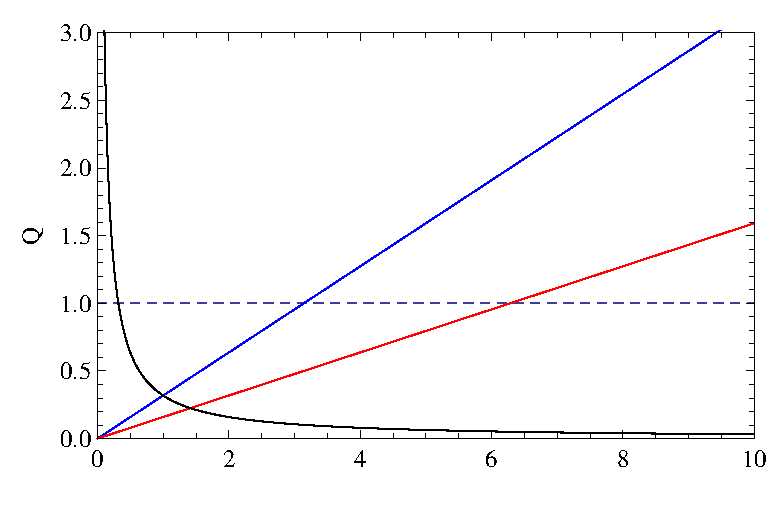
\includegraphics[width=3in]{qplot.eps}
	\caption{This figure qualitatively shows how the Toomre $Q$ parameter changes with respect to $\sigma_s, \kappa,$ or $\mu_\text{disk}$ when all other variables are held constant.  The blue line describes how $Q$ changes with respect to $\sigma_s$ when $\kappa = \mu_\text{disk} = 1$, the red line describes how $Q$ changes with respect to $\kappa$ when $2\sigma_s = \mu_\text{disk} = 1$, and the black line describes how $Q$ changes with respect to $\mu_\text{disk}$ when $\sigma_s = \kappa = 1$.  Values of $Q > 1$ allow for gravitational stability, whereas values of $Q \lesssim 1$ show gravitational instability.  Clearly gravitational stability favors high values of $\kappa$ and $\sigma_s$ and low values of $\mu_\text{disk}$. Horizontal-axis values correspond to non-unit specific values of $\sigma_s$, $\kappa$, or $\mu_\text{disk}$. \label{qFig}}
\end{figure}



\subsection{\label{section 3.2} Effects of gravitational Instability}
Gravitational instability is typically seen in young protoplanetary disks which are massive and have large radii.  Once a disk is gravitationally unstable, numerical simulations have determined three possible outcomes of disk evolution.  First, it is possible for the disk to settle into a quasi-steady, ``saturated'' state in which there is a large amount of self-gravitating turbulence and trailing spiral arms carry angular momentum radially outward.  A second possibility is that the disk will exhibit large accretion bursts.  A third, more interesting possibility shows the disk fragmenting into distinct bound objects, such as young planets \cite{armitage2011}.

\subsection{\label{section 3.3} Gravitational Instability and planet formation}
Theoretically, there are two conditions required for gravitational fragmentation to occur.  First, we must find that $Q \lesssim 1$.  Second, it is necessary for the proto-fragment to cool at a sufficiently rapid pace such that the energy delivered via compression can be radiated away.  Simulations have shown disks successfully achieving gravitational instability at around 30 AU when radiation from the central star is not accounted for.  Unfortunately, those simulations show strong spiral arms developing but no tendency to fragment gravitationally, as the disk is incapable of radiating energy at a rapid enough pace.  On the other hand, those simulations which have included the central star's radiation show a disk with the capability of radiating a sufficient quantity of energy for fragmentation to occur, but such disks are not gravitationally instable at small radii \cite{whitworth2007}.

That being said, it has been shown that Sun-like stars occasionally form with massive, extended protoplanetary disks.  In such cases, brown dwarfs, planetary mass objects, or low-mass hydrogen-burning stars are likely to form via gravitational instability at the far reaches of the disk.  When brown dwarfs do form from fragmentation, they are often liberated from the inner star's gravitational pull.  Over the course of this liberation, they frequently remove a significant portion of the accretion disk around the original star.  This ``stolen'' material settles into a new stable accretion disk around the young, free brown dwarf.  In fact, a single protoplanetary disk of this sort is capable of creating a large number of brown dwarfs (simulations have shown at least 8 from a single disk).  These liberated stars often find a similarly liberated companion and form double brown dwarf binary systems with low mass ratios \cite{hubber2007}.  



\section{\label{section 4} Further Topics}
While this paper has set up a framework for examining the dynamics and gravitational stability of protoplanetary disks, there are a number of significant topics in disk evolution which were outside of the scope of this summary.  For example, while simple $\alpha$ models of viscosity are useful, there is a large amount of literature on the derivation and effects of more complicated models of $\alpha$.  

Additionally, although here we examined self-gravity and gravitational instability, it is clear that these are but a small contributing factor to the development and fragmentation of protoplanetary disks.  Two particularly notable topics which were outside of the scope of this paper are disk radiation and magnetorotational instability, without which it is impossible to say more about the formation of planets.  For a brief overview of all relevant topics in disk evolution, I refer the reader to ``Dynamics of Protoplanetary Disks'' \cite{armitage2011}.

\bibliography{Bibliography}

\end{document}